\documentclass[12pt]{scrartcl}
\usepackage[sexy]{james}
\usepackage[noend]{algpseudocode}
\setlength {\marginparwidth}{2cm}
\usepackage{answers}
\usepackage{array}
\usepackage{tikz}
\newenvironment{allintypewriter}{\ttfamily}{\par}
\usepackage{listings}
\usepackage{xcolor}
\usetikzlibrary{arrows.meta}
\usepackage{color}
\usepackage{mathtools}
\newcommand{\U}{\mathcal{U}}
\newcommand{\E}{\mathbb{E}}
\usetikzlibrary{arrows}
\Newassociation{hint}{hintitem}{all-hints}
\renewcommand{\solutionextension}{out}
\renewenvironment{hintitem}[1]{\item[\bfseries #1.]}{}
\renewcommand{\O}{\mathcal{O}}
\declaretheorem[style=thmbluebox,name={Chinese Remainder Theorem}]{CRT}
\renewcommand{\theCRT}{\Alph{CRT}}
\setlength\parindent{0pt}
\usepackage{sansmath}
\usepackage{pgfplots}

\usetikzlibrary{automata}
\usetikzlibrary{positioning}  %                 ...positioning nodes
\usetikzlibrary{arrows}       %                 ...customizing arrows
\newcommand{\eqdef}{=\vcentcolon}
\newcommand{\tr}{{\rm tr\ }}
\newcommand{\im}{{\rm Im\ }}
\newcommand{\spann}{{\rm span\ }}
\newcommand{\Col}{{\rm Col\ }}
\newcommand{\Row}{{\rm Row\ }}
\newcommand{\dint}{\displaystyle\int}
\newcommand{\dt}{\ {\rm d }t}
\newcommand{\PP}{\mathbb{P}}
\newcommand{\horizontal}{\par\noindent\rule{\textwidth}{0.4pt}}
\usepackage[top=3cm,left=3cm,right=3cm,bottom=3cm]{geometry}
\newcommand{\mref}[3][red]{\hypersetup{linkcolor=#1}\cref{#2}{#3}\hypersetup{linkcolor=blue}}%<<<changed

\tikzset{node distance=4.5cm, % Minimum distance between two nodes. Change if necessary.
         every state/.style={ % Sets the properties for each state
           semithick,
           fill=cyan!40},
         initial text={},     % No label on start arrow
         double distance=4pt, % Adjust appearance of accept states
         every edge/.style={  % Sets the properties for each transition
         draw,
           ->,>=stealth',     % Makes edges directed with bold arrowheads
           auto,
           semithick}}


% Start of document.
\newcommand{\sep}{\hspace*{.5em}}

\pgfplotsset{compat=1.18}
\begin{document}
\title{AMSC460: Homework 5}
\author{James Zhang\thanks{Email: \mailto{jzhang72@terpmail.umd.edu}}}
\date{\today}

\definecolor{dkgreen}{rgb}{0,0.6,0}
\definecolor{gray}{rgb}{0.5,0.5,0.5}
\definecolor{mauve}{rgb}{0.58,0,0.82}

\lstset{frame=tb,
  language=Java,
  aboveskip=3mm,
  belowskip=3mm,
  showstringspaces=false,
  columns=flexible,
  basicstyle={\small\ttfamily},
  numbers=left,
  numberstyle=\tiny\color{gray},
  keywordstyle=\color{blue},
  commentstyle=\color{dkgreen},
  stringstyle=\color{mauve},
  breaklines=true,
  breakatwhitespace=true,
  tabsize=3
}

\maketitle

\begin{center}
  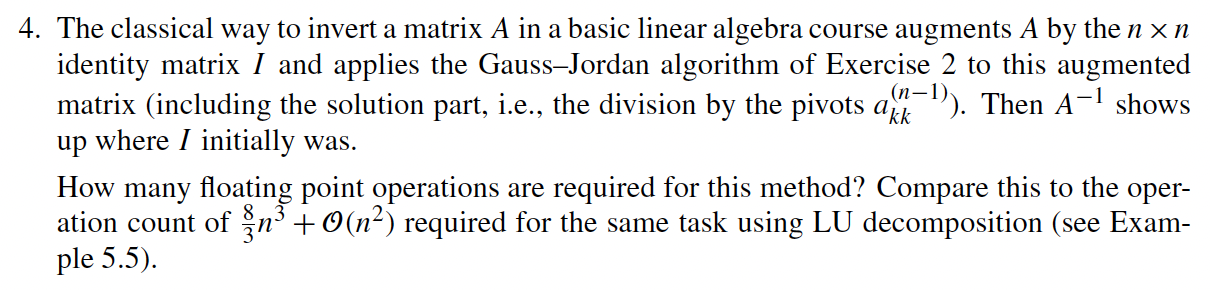
\includegraphics[width=14cm]{4.png}
\end{center}

\begin{proof}
  For the $i$-th row, we essentially need to zero out the other $n-1$ row values in the same column. 
  For each of these $n-1$ subsequent rows, we need to multiply/divide the $j$-th row by a scalar, and then add/subtract 
  from the rows, and we need to do this for both the original matrix and the new matrix which will become the inverse. 
  \[\sum_{i=1}^n (n-i+ 1+ n - i + 1 + n + n + 1 + n)(n - 1) + 2n = + \sum_{i=1}^n (5n - 2i + 2)(n-1) + 2n\]
  where, to clarify, 
  \begin{itemize}
    \item in the first parenthetical expression, suppose we are at the $i$-th row, and we want to zero out all terms below it. Consider the $j$-th row, $j > i$. 
    Then we need to multiply the remaining $n - i$ nonzero elements in the $j$-th row by some scalar. 
    \item Now add/subtract the scaled $n-i+1$ values elementwise to the current $i$-th column
    \item In the soon-to-be identity, we cannot ignore previous columns, and so the multiplications and additions/subtractions 
    must be done to all $n$ elements in each of the rows, so another $n + n$
    \item The last $1$ represents dividing by the pivot, and the $n$ represents this same row transformation to the soon-to-be inverse
    \item Finally, for each row, take the dot product of the newfound row of the inverse by \textbf{b} to get $x_i$ in \textbf{x}, our solution vector
    \item Repeat this process for all necessary $n-i$ rows, and then sum from $1$ to $n$
  \end{itemize}
  \[= \sum_{i=1}^n (5n - 2i + 2)(n-1) + 2n\]
  \[= \sum_{i=1}^n 5n^2 - 5n - 2in + 2i + 2n - 2 + 2n\]
  Simplifying like terms,
  \[= \sum_{i=1}^n 5n^2 - 2in - n + 2i - 2\]
  Breaking up the summation
  \[= 5n^3 - n^2 - 2n - (2n - 2)\left(\sum_{i=1}^n i\right)\]
  \[= 5n^3- n^2 -2n - (2n-2)\frac{n(n+1)}{2}\]
  \[= 4n^3 + \mathcal{O}(n^2)\]
  which is far slower than the LU decomposition method. 
\end{proof}
\newpage

\begin{center}
  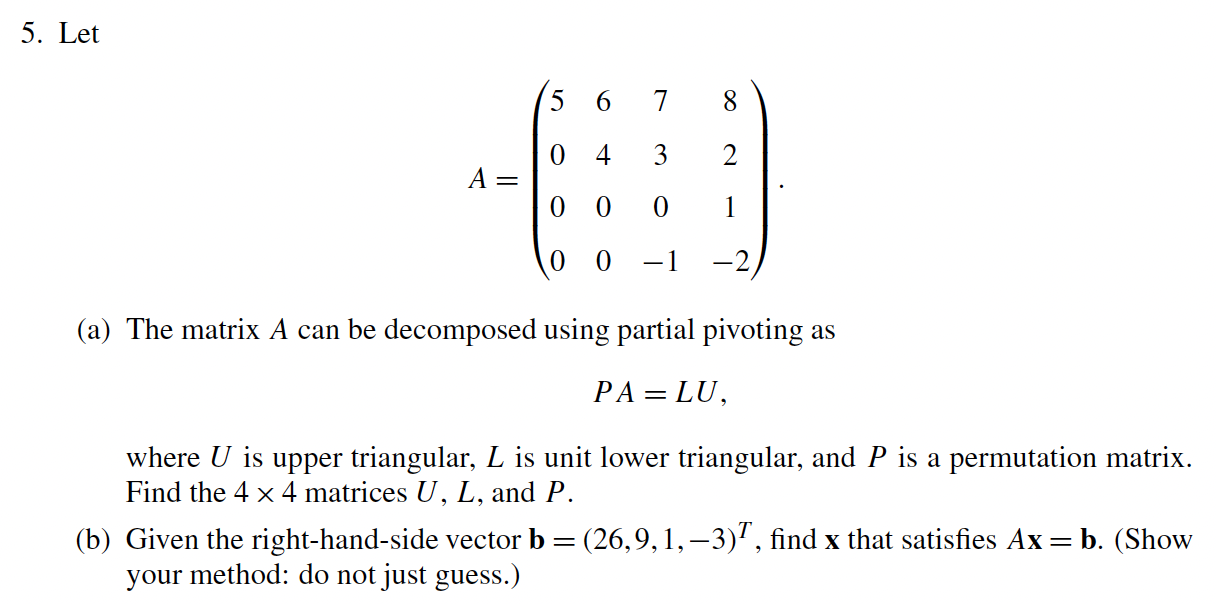
\includegraphics[width=14cm]{5.png}
\end{center}

\begin{proof}
  \hfill

  \begin{enumerate}[(a)]
  \item Let $P^{(1)}$ and $M^{(1)}$ be the $I_4$, as there is no need for partial pivoting in the first column or zero'ing out the first column.
  Thus, $A^{(1)} = M^{(1)}P^{(1)} = A$. Similarly, for the second column, we have 
  $A^{(2)} = M^{(2)}P^{(2)}M^{(1)}P^{(1)} =A$. In the third column, we must switch the third and the fourth row, such that 
  \[P^{(3)} = \begin{bmatrix}
    1 & 0 & 0 & 0\\
    0 & 1 & 0 & 0\\
    0 & 0 & 0 & 1\\
    0 & 0 & 1 & 0
  \end{bmatrix}\]
  $M^{(3)} = I_4$ since there is already a $0$ in the below entry due to the swapping of the rows done by the permutation matrix. 
  Thus, 
  \[U = M^{(3)}P^{(3)}M^{(2)}P^{(2)}M^{(1)}P^{(1)}A= P^{(3)}A = \begin{bmatrix}
    5 & 6 & 7 & 8\\
    0 & 4 & 3 & 2\\
    0 & 0 & -1 & -2\\
    0 & 0 & 0 & 1
  \end{bmatrix}\]
  Given all of the permutation matrices, we can now calculate $P$ which is 
  \[P = P^{(3)}P^{(2)}P^{(1)} = P^{(3)} = \begin{bmatrix}
    1 & 0 & 0 & 0\\
    0 & 1 & 0 & 0\\
    0 & 0 & 0 & 1\\
    0 & 0 & 1 & 0
  \end{bmatrix}\]
  Finally, since $L = P(M^{(3)}P^{(3)}M^{(2)}P^{(2)}M^{(1)}P^{(1)})^{-1}$, this 
  nicely simplifies to 
  \[L = P^{(3)}P^{(3)} = I_4 = \begin{bmatrix}
    1 & 0 & 0 & 0\\
    0 & 1 & 0 & 0\\
    0 & 0 & 1 & 0\\
    0 & 0 & 0 & 1
  \end{bmatrix}\]
  \item Note that $P = P^{(3)}$ and that $(P^{(3)})^{-1} = P^{(3)}$, observe that 
  \[PA = LU \implies P^{-1}PA = P^{-1}LU \implies A = PLU\]
  Thus, we want to find $\textbf{x}$ such that $PLU\textbf{x} = \textbf{b} = (26, 9, 1, -3)^T$. Note that 
  \[PLU\textbf{x} = \textbf{b} \implies LU\textbf{x} = P\textbf{b} = (26, 9, -3, 1)^T\]
  Now, we can proceed with forward and backward substitution. Let $\textbf{y} = U\textbf{x}$. We seek 
  $\textbf{y}$ such that 
  \[L\textbf{y} = (26, 9, -3, 1)^T \implies \textbf{y} = (26, 9, -3, 1)^T\]
  because $L = I_4$. Now we seek the original $\textbf{x}$ such that
  \[U\textbf{x} = \begin{bmatrix}
    5 & 6 & 7 & 8\\
    0 & 4 & 3 & 2\\
    0 & 0 & -1 & -2\\
    0 & 0 & 0 & 1
  \end{bmatrix}\begin{bmatrix}
    x_1 \\ x_2 \\ x_3 \\ x_4
  \end{bmatrix}= \begin{bmatrix}
    26 \\ 9 \\ -3 \\ 1
  \end{bmatrix}\]
  By backward substitution, $x_4 = 1 \implies -x_3 - 2 = -3 \implies x_3 = 1$, and continuining in this manner 
  yields 
  \[\textbf{x} = \begin{bmatrix}
    1 \\ 1 \\ 1 \\ 1
  \end{bmatrix}\]
  \end{enumerate}
\end{proof}
\newpage

\begin{center}
  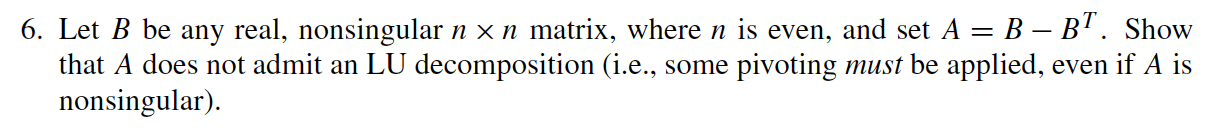
\includegraphics[width=14cm]{6.png}
\end{center}

\begin{proof}
  Note that $A = B - B^T$ omits the following form
  \[A = \begin{bmatrix}
    0 & a & b & \cdots & A_{1n}\\
    -a & 0 & c & \cdots & A_{2n}\\
    -b & -c & 0 & \cdots & A_{3n}\\
    \vdots & \vdots & \vdots & \ddots & \vdots\\
    -A_{1n} & -A_{2n} & -A_{3n} & \cdots & 0
  \end{bmatrix}\]
  where this is known as a \textbf{skew symmetric matrix}, which have the property that $A^T = -A$. Furthermore, recall that if a square matrix $X$ is invertible, then $\det(A) = \det(A^T)$. 
  We will show that a skew symmetric square matrix $X \in \RR^{n' \times n'}$, where $n'$ is odd, must have $\det(X) = 0$. 
  \[X^T = -X \implies \det(X^T) = \det(-X) \implies \det(X^T) = (-1)^{n'} \det(X)\]
  This last equation can only be satisfied if $\det(X) = \det(X^T) = 0$. Thus, any odd-sized square symmetric matrix 
  is singular. In the context of our problem, while $A$ need not be singular, its odd-sized principal minors -- the smaller square submatrices -- 
  must be singular, and so there does not exist an LU decomposition of $A$ without pivoting. 
\end{proof}
\end{document}

